\begin{figure}[t]
\centering
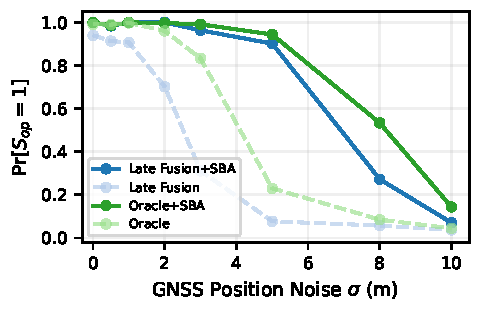
\includegraphics[width=\columnwidth]{figures/gnss_noise_robustness.pdf}
\caption{Operational success vs.\ GNSS position noise (standard deviation $\sigma$ in metres), at 200\,ms configured latency with $N{=}1$. Without SBA (left), spatial-only self-identification degrades rapidly once $\sigma$ exceeds ${\sim}2\,\mathrm{m}$. With SBA (right), the beacon carries an authoritative identity that does not depend on position accuracy, and operational success remains high until $\sigma$ exceeds ${\sim}5\,\mathrm{m}$.}
\label{fig:gnss_robustness}
\end{figure}
